\section{Context of use}
	\subsection{User journey maps}
		For a greater understanding of future design choices and possible requirements, a user journey map for the lending and renting part of the application is created respectively. The different phases a user traverses are defined in the first step. The second step consists of finding possibles activities the user performs in the phases. In the last step the users feelings while performing the activities are depicted. This helps finding possible phases of the journey that may be difficult and finding a solution to simplify these phases.\\
		
		\subsubsection{User journey map for the renting person}
			This journey map consists of the following phases with the related activities:
			
			\begin{figure}[H]
				\centering
				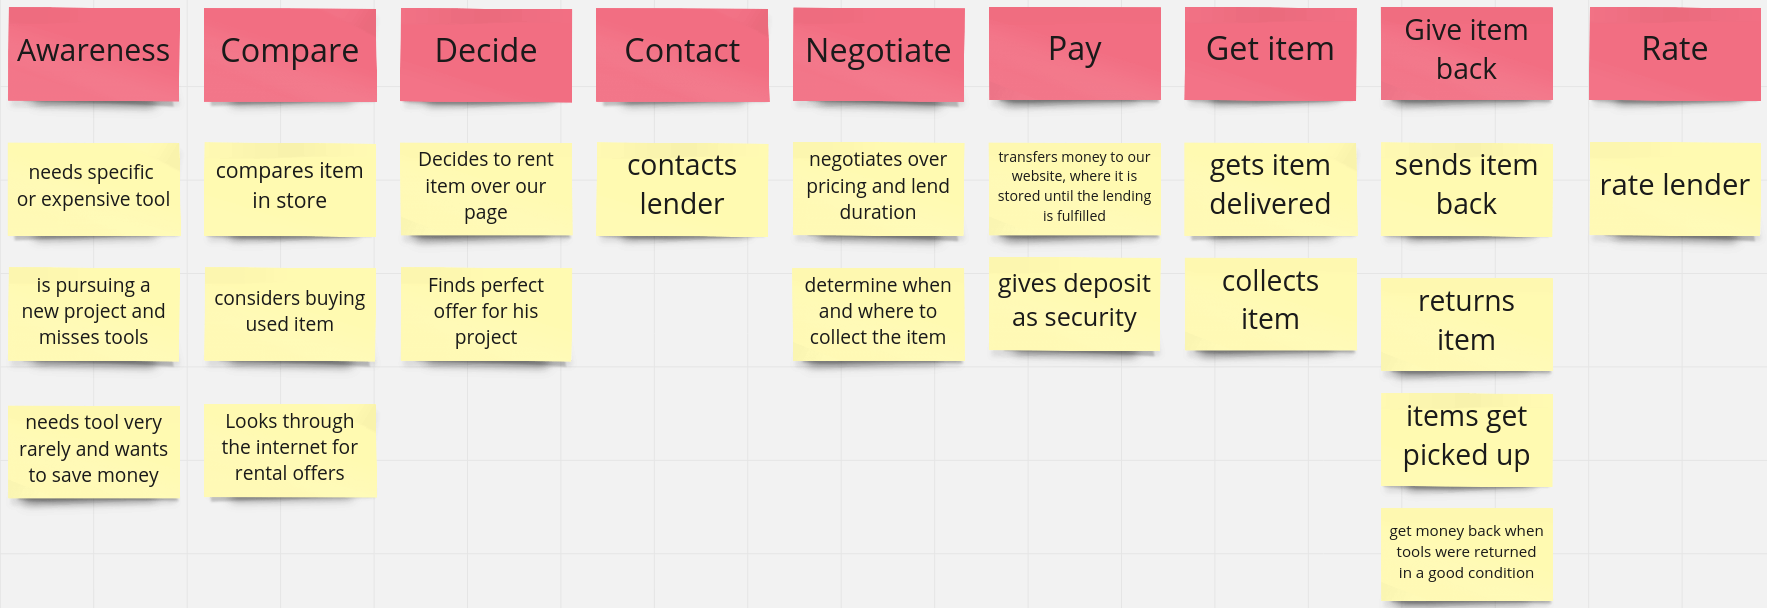
\includegraphics[width=\linewidth]{abb/2_context_of_use/user_journey_map_renting.png}
				\caption{User journey map for renting user}
				\label{fig:ujm_renting}
			\end{figure}
			
			\noindent
			The corresponding feelings and the graph are determined this way:
			
			\begin{figure}[H]
				\centering
				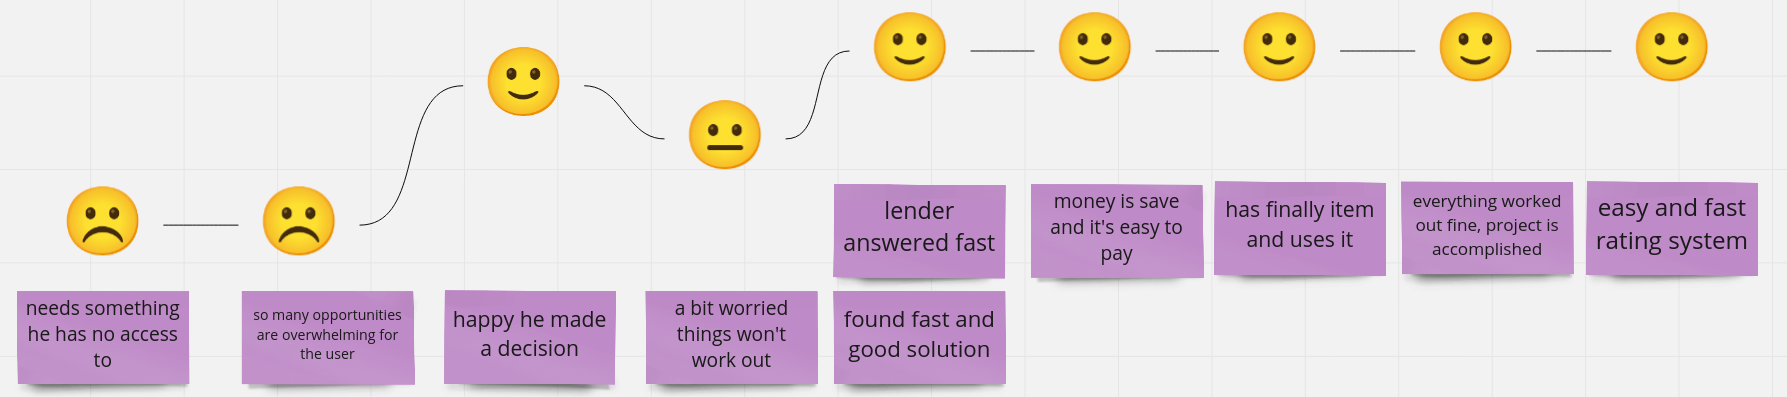
\includegraphics[width=\linewidth]{abb/2_context_of_use/feelings_renting.png}
				\caption{Feelings for renting user}
				\label{fig:ujm_renting_feelings}
			\end{figure}
		
		\subsubsection{User journey map for the renting person}
			The counterparts for the renting persons journey looks like this:
			
			\begin{figure}[H]
				\centering
				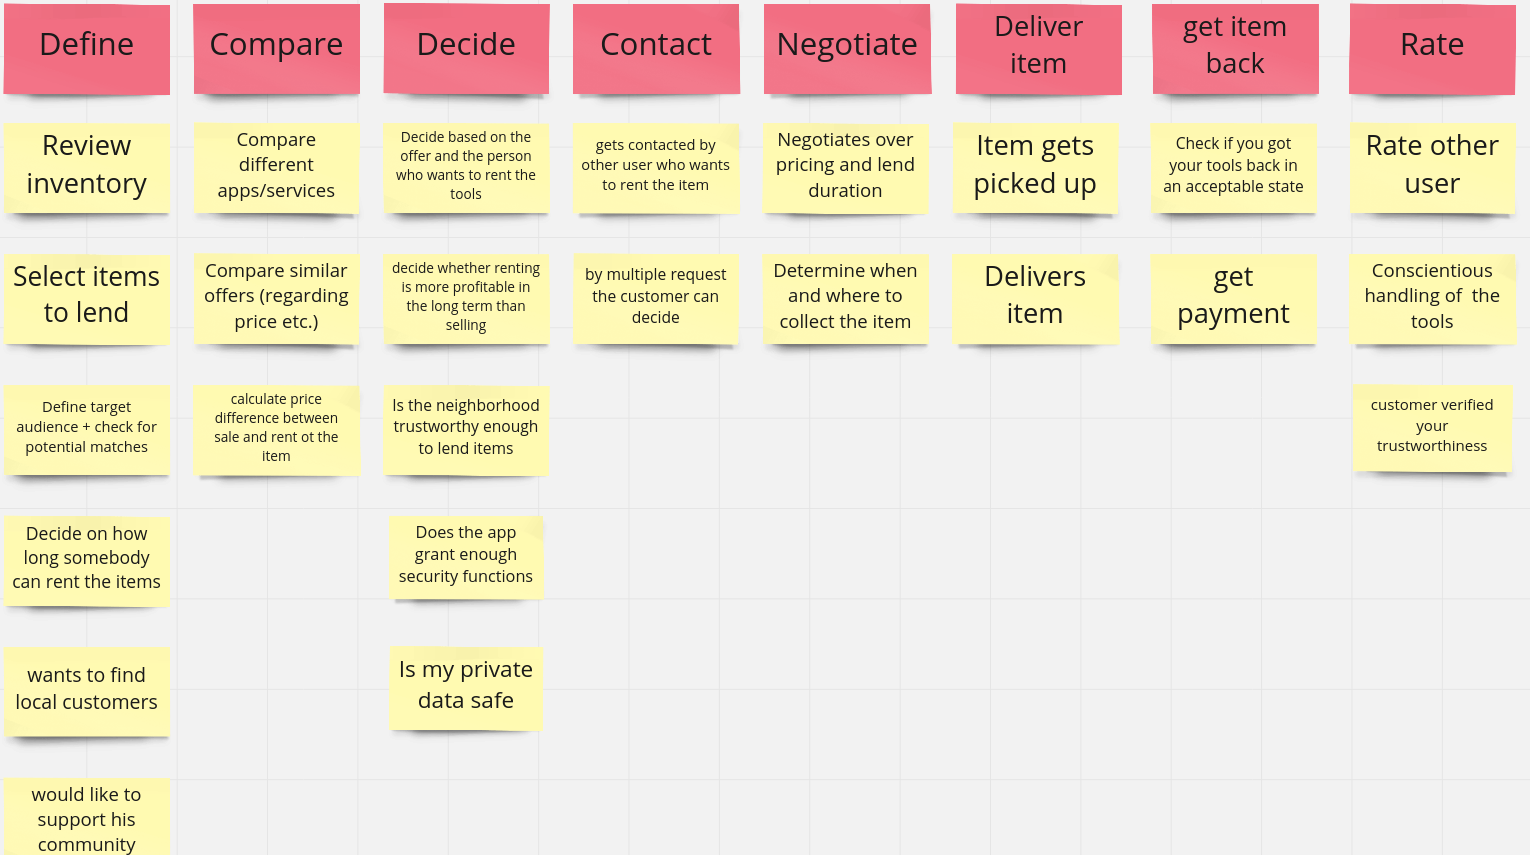
\includegraphics[width=\linewidth]{abb/2_context_of_use/user_journey_map_lending.png}
				\caption{User journey map for lending user}
				\label{fig:ujm_lending}
			\end{figure}
		
			\begin{figure}[H]
				\centering
				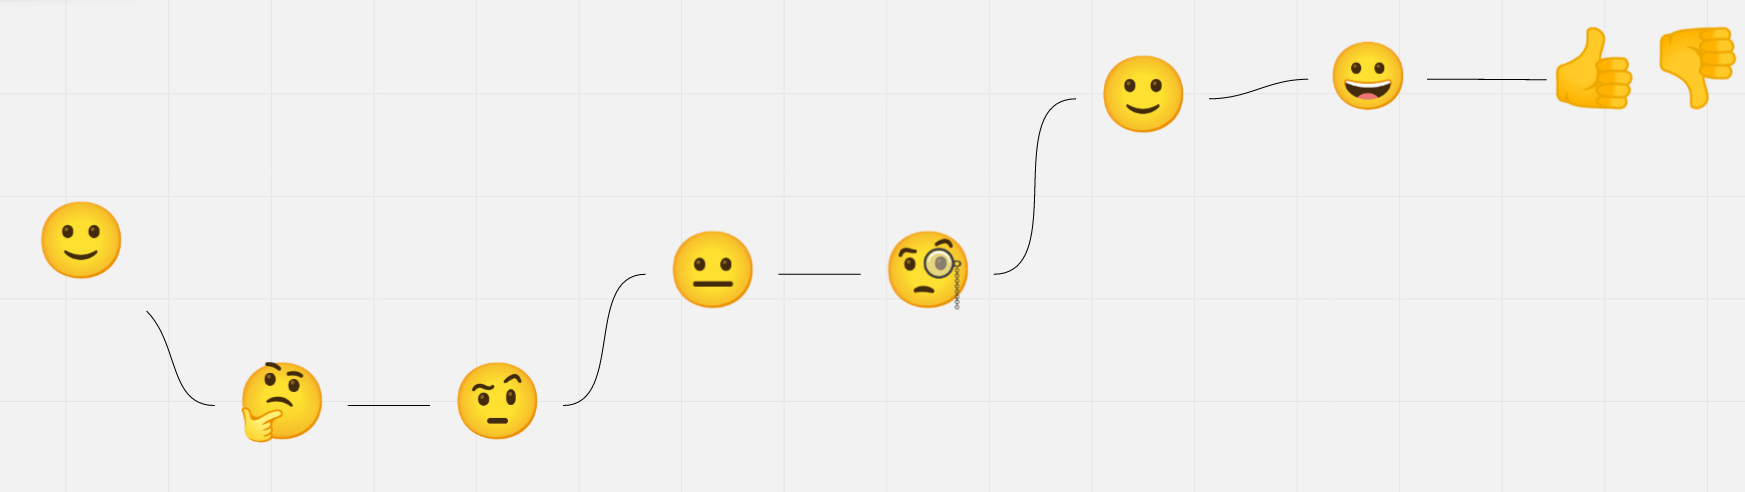
\includegraphics[width=\linewidth]{abb/2_context_of_use/feelings_lending.png}
				\caption{Feelings for renting user}
				\label{fig:ujm_lending_feelings}
			\end{figure}